\section{Einfluss eines Magneten auf eine Aluminiumplatte und auf einen Aluminiumkamm }\label{kap:Kamm_Platte}
Bei diesem Experiment ging es darum das verhalten zweier unterschiedlich geformter Körper aus dem gleichem Material zu untersuchen. Der Versuchsaufbau ist in \cref{fig:Alukamm} zu sehen.
Um das verhalten der Platte und des Kammes zu untersuchen wurde eine Reihe aus drei Magneten einmal schnell auf die Platte zubewegt und wieder entfernt und danach langsam angenähert und langsam wieder entfernt. Diese Aktionen wurden danach bei dem Kamm wiederholt.
Beim schnellen annähern an die Platte schwang die Platte zurück und beim langsamen entfernen wurde sie mitgezogen.
Dieses verhalten ist auf Diamagnetismus beziehungsweise Paramagnetismus zurückzuführen. Beim schnellen annähern tritt der Diamagnetismus auf und die Platte wurde aus dem Magnetfeld verdrängt. Entfernt man die Magneten jedoch langsam wieder überlagern die deutlich stärkeren Paramagnetischen Effekte den Diamagnetismus und die Platte wird mitgezogen.
Das bei dem Kamm nur der Paramagnetismus auftritt und das auch nur sehr schwach ist auf die Unterbrechungen in der Oberfläche zurückzuführen. Diese Unterbrechungen sorgen dafür das die Wirbelströme die auf die Oberfläche induziert werden deutlich schwächer ausfallen als bei der Platte.
Dadurch wird der sowieso schon sehr schwache Diamagnetische Effekt so stark abgeschwächt das er bei einem so schwachen Magnetfeld nicht mehr zu sehen ist.
\begin{figure}[h]
	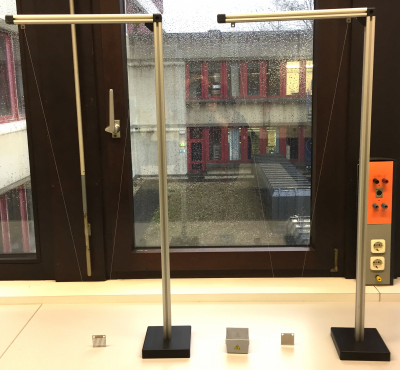
\includegraphics[width=0.5\textwidth]{res/Alupendel.png}
	\caption{In dieser Abbildung ist der Versuchsaufbau zu sehen mit dem man den Einfluss eines Magneten auf eine Aluplatte und auf einen Alukamm untersucht wurde\protect\footnotemark.}
	\label{fig:Alukamm}
\end{figure}
\footnotetext{Entnommen am 20.11.17  aus dem Learnweb Kurs "Experimentelle Übungen I 17-18"}
